\documentclass[11pt,a4paper]{article}

\usepackage[margin=2.2cm]{geometry}
\usepackage{graphicx}
\usepackage{booktabs}
\usepackage{tabularx}
\usepackage{array}
\usepackage{caption}
\usepackage{float}
\usepackage{xcolor}
\usepackage{tikz}
\usepackage[hidelinks]{hyperref}
\usetikzlibrary{arrows.meta, positioning, shapes.geometric}

\graphicspath{{./}{figures/}{../}}

\definecolor{accent}{HTML}{0E6B67}
\definecolor{softgray}{HTML}{F4F6F6}
\definecolor{midgray}{HTML}{666666}
\definecolor{softaccent}{HTML}{E7F4F2}
\definecolor{softgold}{HTML}{FFF4D6}

\setlength{\parindent}{0pt}
\setlength{\parskip}{0.6em}
\renewcommand{\arraystretch}{1.15}
\captionsetup{labelsep=period}
\newcolumntype{L}[1]{>{\raggedright\arraybackslash}p{#1}}
\newcolumntype{Y}{>{\raggedright\arraybackslash}X}
\newcommand{\evidencecard}[2]{
    \fcolorbox{midgray}{softgray}{
        \begin{minipage}{0.95\textwidth}
            \textbf{#1}\\[0.35em]
            \small #2
        \end{minipage}
    }
}

\newcommand{\boxfigure}[3]{
    \begin{figure}[H]
        \centering
        \fcolorbox{midgray}{softgray}{
            \begin{minipage}[c][4.5cm][c]{0.9\textwidth}
                \centering
                \textbf{#1}\\[0.4em]
                \small #2
            \end{minipage}
        }
        \caption{#1.}
        \label{#3}
    \end{figure}
}

\begin{document}
\pagenumbering{gobble}

\begin{titlepage}
    \centering
    \vspace*{0.2cm}
    
\includegraphics[width=4.2cm]{unsw_logo.png}

    \vspace{1.1cm}
    {\Large DESN2000 SENG\par}
    \vspace{0.3cm}
    {\Huge\bfseries Interim Report\par}
    \vspace{0.25cm}


    \vspace{1.2cm}
    \begin{tabular}{@{}ll@{}}
        Project space & Smart Share House \& Student Living Assistant\\
        Team members & Nuodi Liu (z5403196), Qian Cao (z5569891), Chien-Kai, Wang (z5505220), Pranav (z5589687)\\
    \end{tabular}

    \vfill
\end{titlepage}

\pagenumbering{roman}
\tableofcontents
\newpage
\pagenumbering{arabic}

\section{Introduction and Project Context}

Shared accommodation is a common housing option for university students, especially international students and those living away from home for the first time. However, searching for accommodation and suitable housemates can be difficult, since students often have limited information when making their decision. Our initial research showed that many problems occur before moving in, including concerns about trustworthy listings, communication, and housemate compatibility. This report explores these issues through user research and stakeholder analysis to better understand students' needs and identify opportunities for improving the shared accommodation experience.

\section{Stakeholders}

Stakeholder mapping helped the team identify the groups affected by shared living and then focus on users who face the greatest uncertainty when accommodation decisions are made.

\begin{table}[H]
    \centering
    \small
    \caption{Stakeholder priority and impact summary.}
    \begin{tabularx}{\textwidth}{@{}L{2.7cm} Y Y L{1.9cm} L{2.4cm}@{}}
        \toprule
        Stakeholder & Needs & Impact if unmet & Priority & Evidence source\\
        \midrule
        International students & They need listings they can trust, rental information they can understand and housemates who fit their routines. & They may face scams, choose unsuitable housing or feel stressed before arrival. & Primary & Survey and interview\\
        Existing housemates & They need applicants who are reliable, tidy and respectful. & The household may experience conflict, unpaid bills and uneven responsibility sharing. & Primary & Survey and interview\\
        Domestic students & They need simple ways to discuss household work, bills and communication. & Shared living can become tense, and social connection may weaken. & Primary & Domestic survey\\
        Property managers & They need enquiries that are easier to handle and applicants who provide enough information. & They may deal with repeated messages and incomplete applications. & Secondary & Persona analysis\\
        \bottomrule
    \end{tabularx}
    \label{tabstakeholders}
\end{table}

International students, existing housemates and domestic students were prioritised because these groups carry substantial risk at different points in the shared living experience. International students must judge unfamiliar listings and rental norms, existing housemates must live with the consequences of poor housemate matching, and domestic students show how unclear household responsibilities can create conflict after move in. Property managers were treated as secondary stakeholders because they shape listing trust and communication, but they are not the main users of the proposed student living support system.

\section{Research Methods and Synthesis}

The team used mixed methods to identify common patterns and understand why those patterns matter in everyday shared living. Surveys showed the scale of recurring concerns, while the interview and persona work gave context to the decisions students make when choosing accommodation or housemates.

The research questions examined how students judge whether a listing can be trusted, what they need to know before contacting a landlord or housemate, which qualities shape housemate fit and how shared responsibilities can create conflict after move in.

\begin{table}[H]
    \centering
    \small
    \caption{Research question focus areas.}
    \begin{tabularx}{\textwidth}{@{}L{3.2cm} Y@{}}
        \toprule
        Focus area & Example research question\\
        \midrule
        Trust & How concerned are students about rental scams, fake listings or misleading housing information?\\
        Compatibility & How important is roommate compatibility when students choose accommodation?\\
        Communication & What information do students need before they decide whether to make contact or commit?\\
        Shared responsibilities & How are household work, bills and house rules handled after move in?\\
        \bottomrule
    \end{tabularx}
    \label{tabresearchquestions}
\end{table}

\begin{table}[H]
    \centering
    \small
    \caption{Research methods used during the Empathise stage.}
    \begin{tabularx}{\textwidth}{@{}L{3.0cm} L{3.3cm} Y Y@{}}
        \toprule
        Method & Participants or source & Purpose & Output used in report\\
        \midrule
        International student survey & 16 valid responses & Understand accommodation search concerns, with attention to scams, communication and compatibility. & Charts and theme counts\\
        Domestic student survey & 3 students in shared accommodation & Understand problems that appear after move in, such as household work, bills and conflict. & Shared living pain points\\
        Student interview & 1 participant & Explore trust, cleanliness, privacy and housemate expectations in more depth. & Qualitative validation\\
        Persona and stakeholder analysis & Team persona files & Turn research evidence into user archetypes. & Personas, scenarios and journey maps\\
        Affinity mapping and mind map & Team synthesis artefact & Group findings and compare them by frequency, severity and design relevance. & Final themes and problem definition\\
        \bottomrule
    \end{tabularx}
    \label{tabmethods}
\end{table}

The questionnaire data was summarised by comparing frequency, severity and design relevance. The international survey had a larger sample and was used to identify accommodation search risks before commitment. The domestic survey had a smaller sample, so it was treated as supporting evidence for problems that appear after move in rather than as a generalisable result.

\begin{table}[H]
    \centering
    \small
    \caption{Questionnaire insight summary and design relevance.}
    \begin{tabularx}{\textwidth}{@{}L{3.1cm} Y Y@{}}
        \toprule
        Evidence pattern & Survey result & Design relevance\\
        \midrule
        Search channels are fragmented & International students most often used third-party housing platforms (37.5\%) and student social media groups (25\%). & Trust support should work across informal and platform-based search behaviours.\\
        Pre-arrival uncertainty is practical & Language barriers were the most selected pre-arrival difficulty (43.75\%), and 68.75\% took one to four weeks to find suitable accommodation. & Listing pages and messages should explain key information clearly and reduce decision friction.\\
        Trust is a universal concern & 100\% of international respondents were concerned about scams, and 43.75\% had experienced misleading or false housing advertisements. & Verification, reviews and safer contact flows should be core features rather than optional extras.\\
        Compatibility is measurable & 87.5\% of international respondents rated roommate compatibility as very or extremely important. & Matching should compare concrete routines and expectations, not only demographic information.\\
        Informal systems create conflict & In the domestic survey, 100\% used verbal chore agreements, 100\% had conflict over household responsibilities and 66.67\% had no formal bill-splitting arrangement. & Shared responsibility expectations should be visible before move in and trackable after move in.\\
        Current tools are incomplete & Domestic respondents used mobile group chat (100\%) but no chore management app, while 100\% reported issues with housemates not paying expenses on time. & The product should combine communication, chores and expense accountability in one workflow.\\
        \bottomrule
    \end{tabularx}
    \label{tabsurveyinsights}
\end{table}

After data collection, the team used affinity mapping to group repeated observations. Five themes emerged across the evidence. The strongest pattern was that worries about trust and uncertainty about compatibility appear before commitment, yet they often shape conflict after students move in.

\begin{figure}[H]
    \centering
    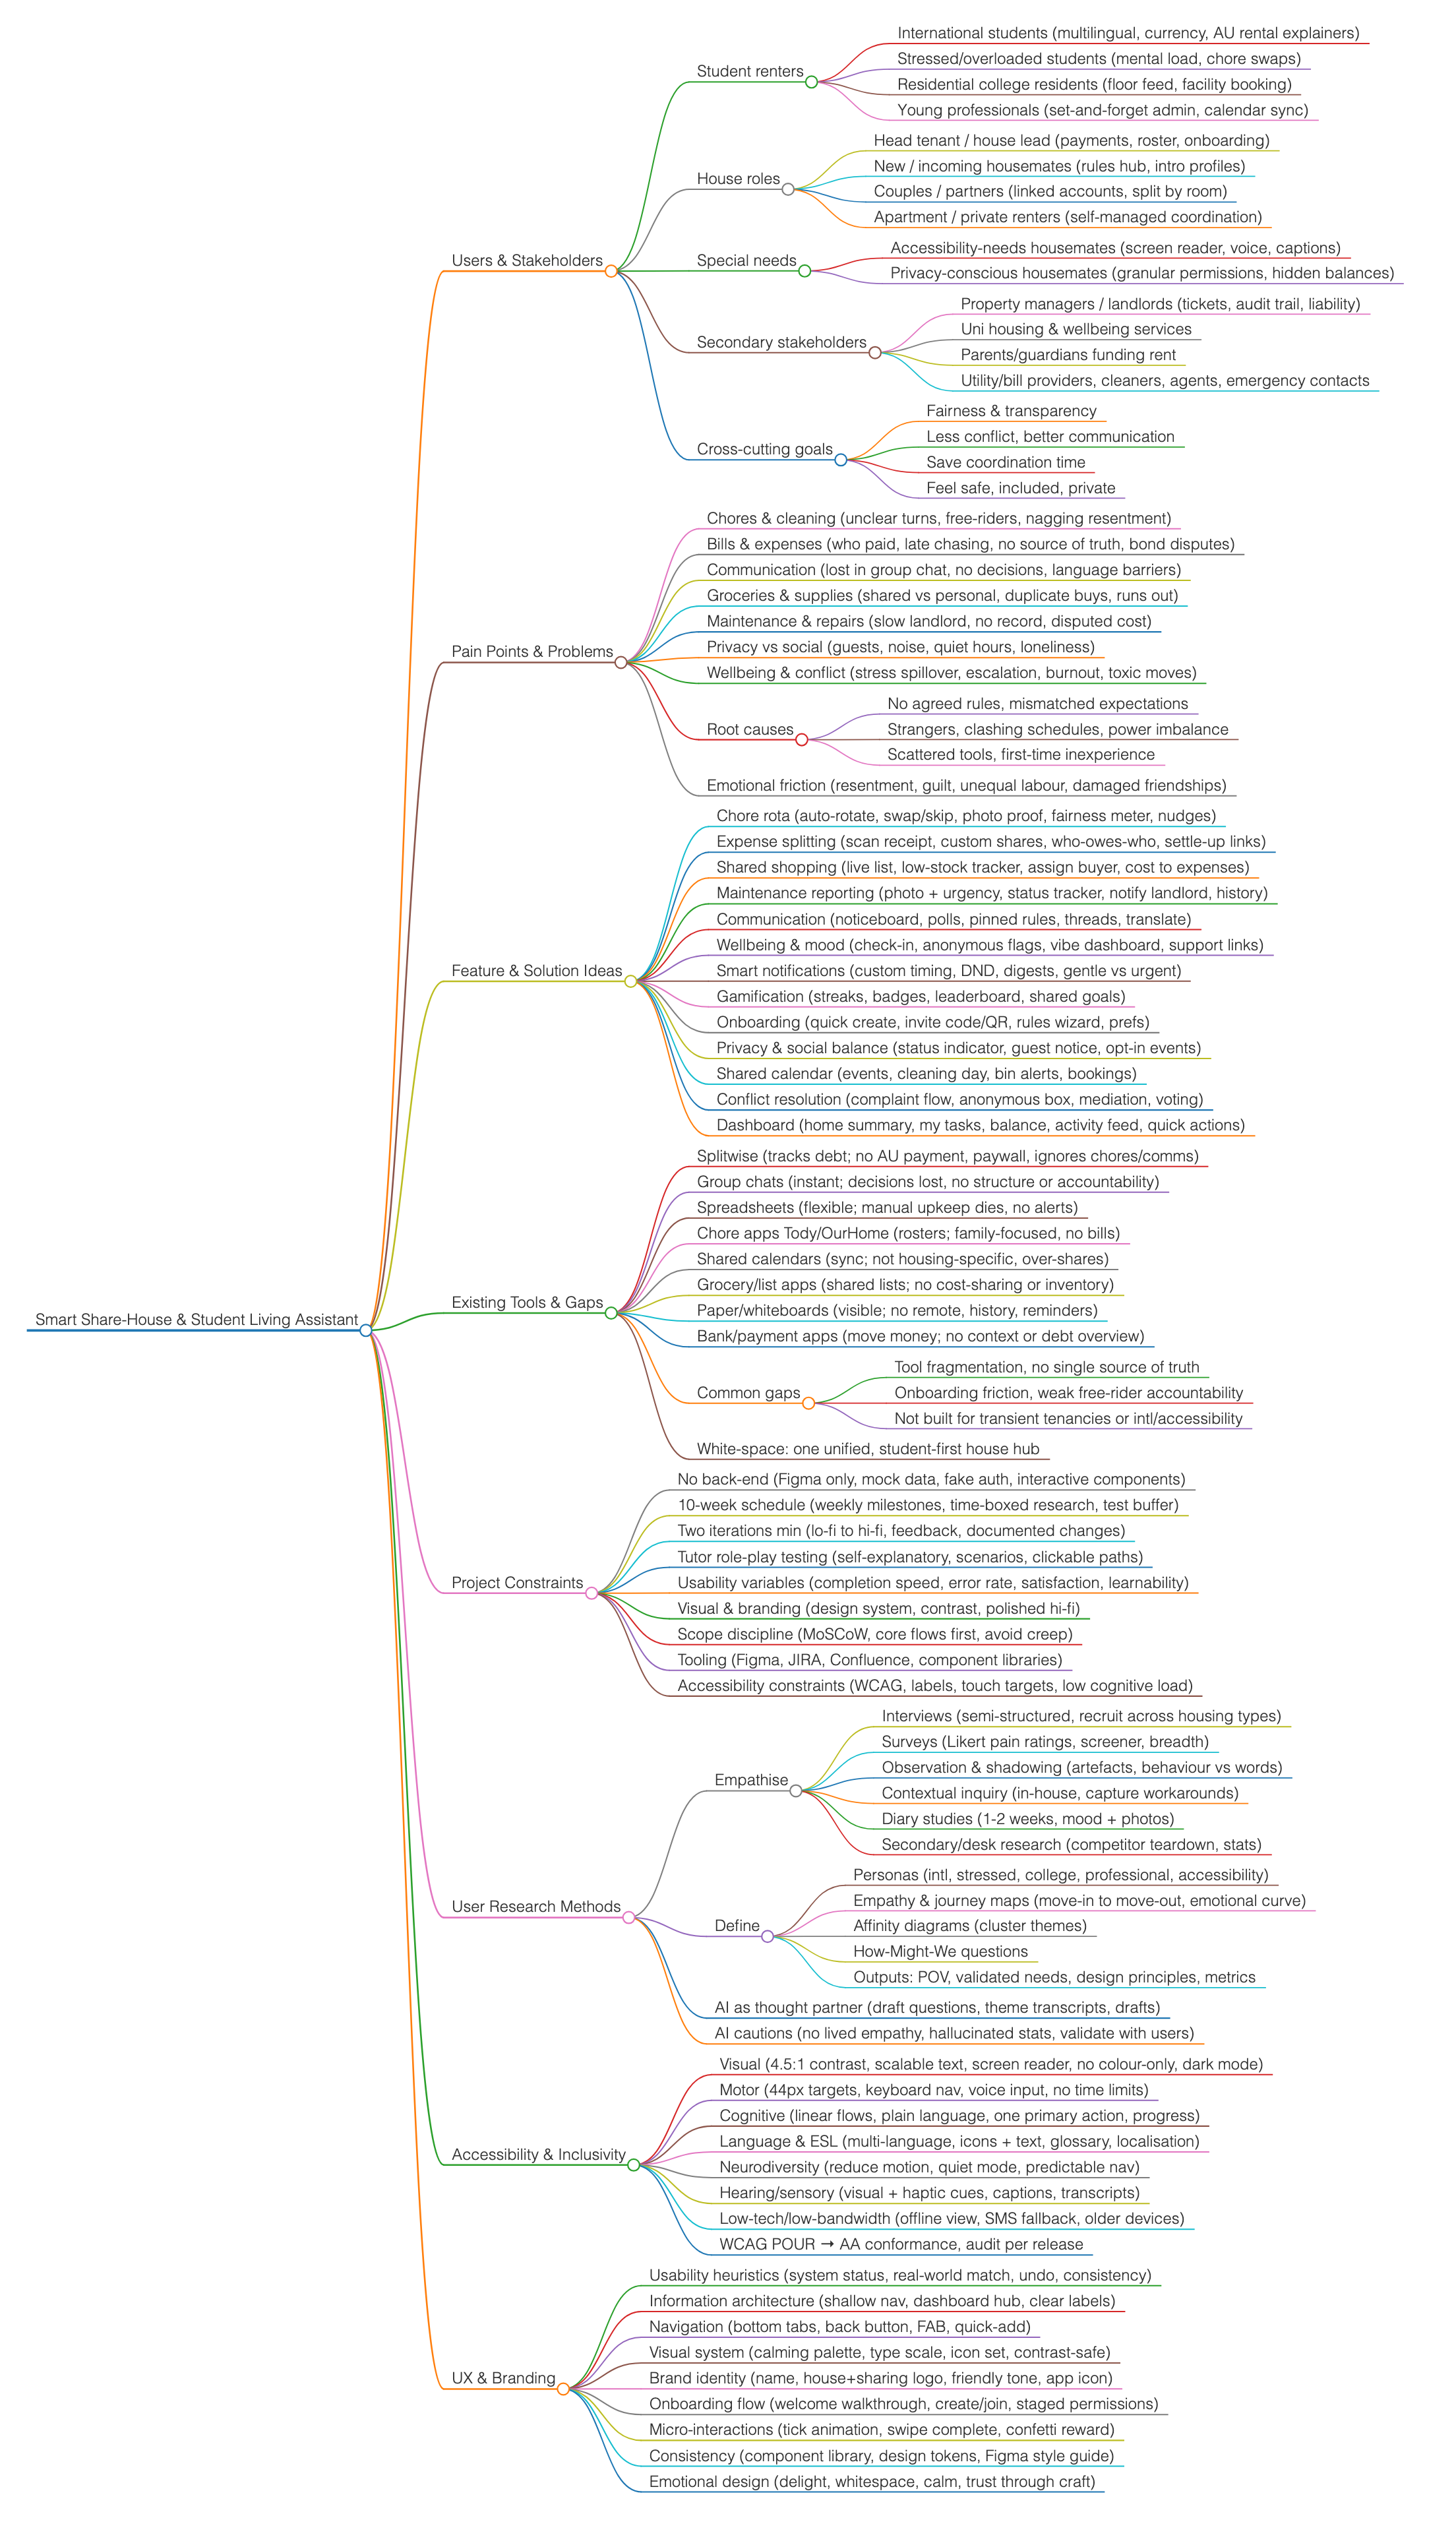
\includegraphics[width=\textwidth,height=0.5\textheight,keepaspectratio]{mindmap.png}
    \caption{Affinity map and mind map showing research themes from survey, interview and team synthesis.}
    \label{figaffinity}
\end{figure}

\section{Key Research Findings}

\subsection{Trust and Safety Shape Accommodation Decisions}

All 16 international student survey respondents reported concern about rental scams, with half being very concerned and half being slightly concerned. The survey also showed that 43.75\% had experienced misleading or false information in a housing advertisement. Students used mixed search channels, including third-party housing platforms (37.5\%) and social media groups (25\%), which increases the need for consistent trust cues across informal and formal search contexts. This suggests that students do not only need access to more listings. They need help checking the person who posted a listing, matching the photos with the room and keeping early messages inside a safer platform. Student feedback should also be easy to find.

\begin{figure}[H]
    \centering
    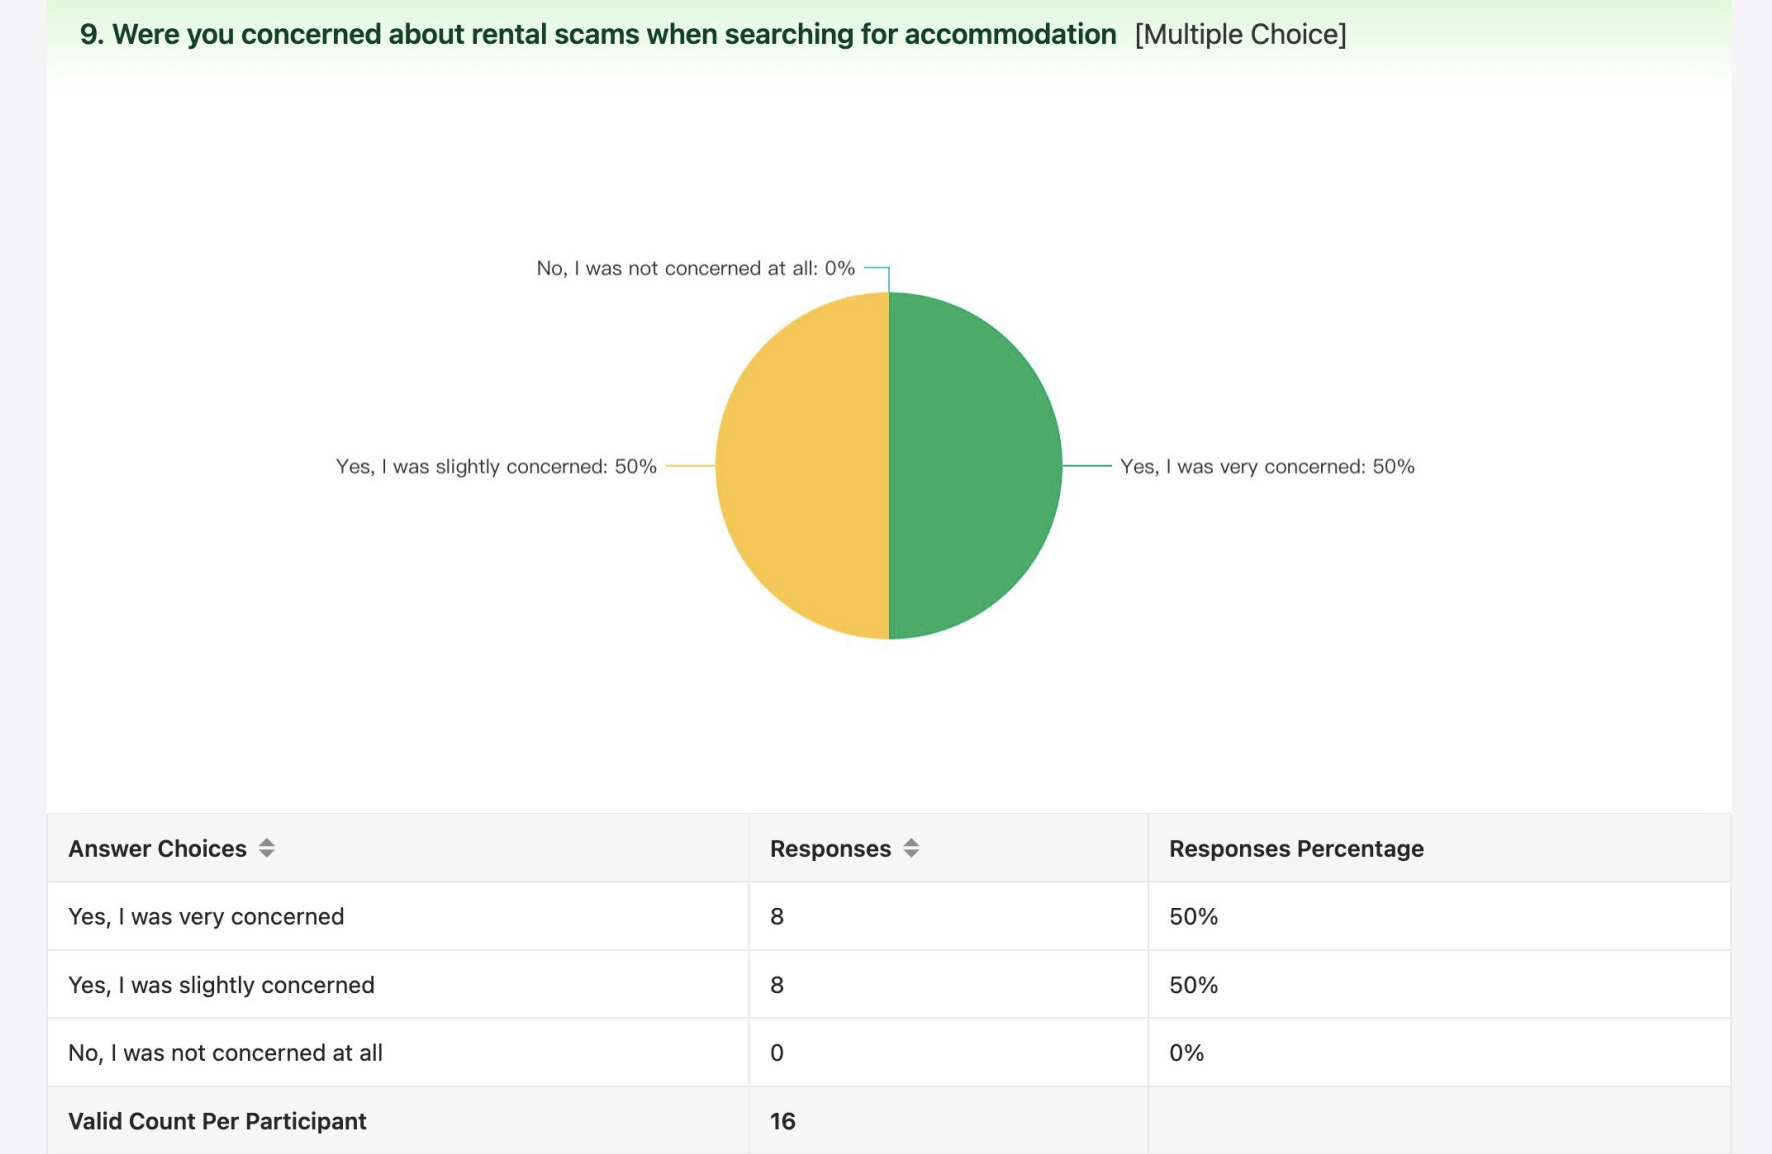
\includegraphics[width=0.94\textwidth]{survey_scams_concern.png}
    \caption{International student survey result. Concern about rental scams, n=16.}
    \label{figscams}
\end{figure}

\subsection{Housemate Compatibility Is a High Priority Decision Factor}

The international student survey showed an average roommate compatibility importance score of 4.44 out of 5, with 87.5\% rating compatibility as very or extremely important. The most selected roommate qualities were quiet and respectful rest time (62.5\%), non-smoker and non-drinker (62.5\%), clean and tidy habits (56.25\%), similar daily schedule (50\%) and willingness to share housework responsibilities (50\%). The interview also showed that compatibility is practical rather than abstract. Students wanted to know whether housemates keep spaces clean, respect privacy and follow routines that would not clash with their own. The design should make this information visible before users commit to a room.

\begin{figure}[H]
    \centering
    
\includegraphics[width=0.94\textwidth]{survey_roommate_compatibility.png}
    \caption{International student survey result. Roommate compatibility importance, n=16.}
    \label{figcompatibility}
\end{figure}

\subsection{Communication and Information Gaps Increase Uncertainty}

International students may not know Australian rental processes, inspection expectations or the cues used to judge whether a listing is reliable. In the international survey, language barriers were the most selected difficulty before arrival (43.75\%), while 68.75\% of respondents took between one and four weeks to find suitable accommodation. The interview participant wanted to see where the room was, what it looked like in realistic photos, whether reviews were available and what facilities were nearby. This points to a need for listing pages and messages that guide the user through a decision rather than leaving them to interpret scattered information on their own.

\begin{figure}[H]
    \centering
    
\includegraphics[width=0.94\textwidth]{survey_search_challenges.png}
    \caption{International student survey result. Accommodation search challenges before arrival, n=16.}
    \label{figbarriers}
\end{figure}

\subsection{Shared Living Conflicts Often Come From Unclear Expectations}

Domestic student findings showed that informal household systems can fail after move in. Although the domestic survey was small, all respondents relied on verbal agreements for household work, and all had experienced conflict over household responsibilities. Bill splitting was also weakly structured, as 66.67\% reported no formal arrangement and all reported issues with housemates not paying expenses on time. Communication was concentrated in mobile group chat (100\%), while no respondent used a chore management app. The design should help students discuss responsibility expectations before move in and then keep those expectations visible after move in, rather than relying only on personality matching.

\begin{figure}[H]
    \centering
    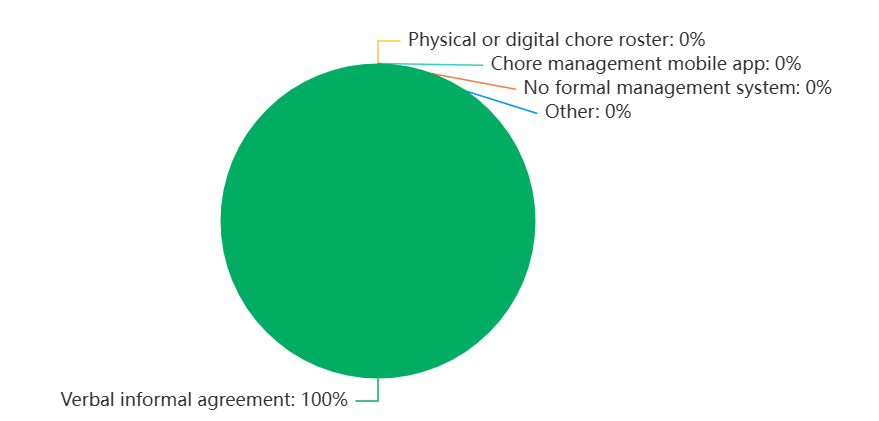
\includegraphics[width=0.82\textwidth]{domestic_chore_methods.png}
    \caption{Domestic student survey result. Household work management methods, n=3.}
    \label{figchores}
\end{figure}

\begin{figure}[H]
    \centering
    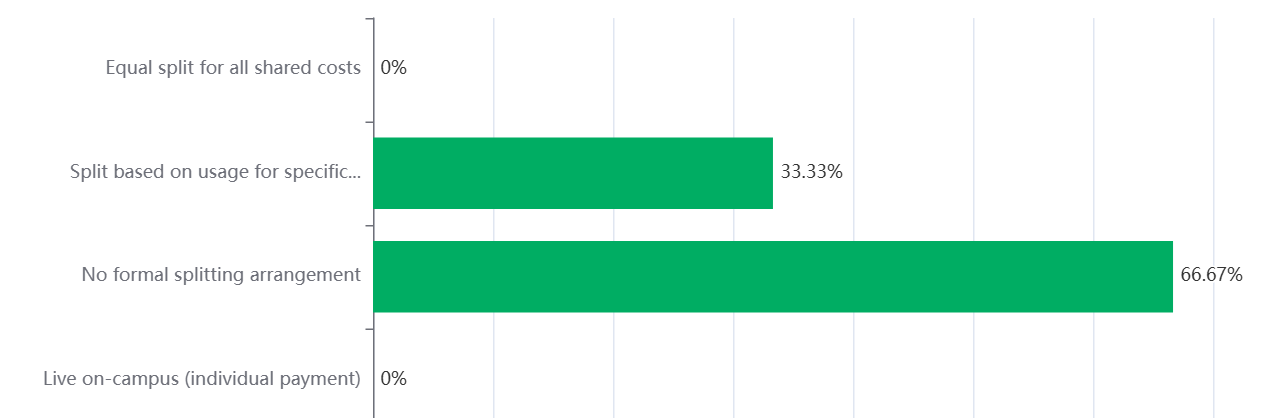
\includegraphics[width=0.94\textwidth]{domestic_bill_splitting.png}
    \caption{Domestic student survey result. Bill splitting arrangements, n=3.}
    \label{figbills}
\end{figure}

\section{Personas, Scenarios and Journey Maps}

The four personas were developed from survey findings, interview insights and team synthesis artefacts. They were used to turn repeated research themes into concrete user situations, rather than treating users as abstract groups. Together, the personas show how different stakeholders experience the accommodation decision process from different positions. International students face uncertainty when judging unfamiliar listings before arrival. Emily Chen represents a general resident perspective, where the main concern is whether a new person will fit into an existing household. Domestic students already living in shared accommodation reveal how unclear agreements around chores, bills and house rules can become conflict after move in. Property managers show the operational constraints around listing trust, enquiry handling and applicant screening.

Across the four personas, the strongest pattern is that users need clearer information before they make or accept a commitment. Trust, compatibility, communication and shared responsibility expectations appear in different ways for each persona, but they all affect the same decision point. Users are often asked to choose a room, contact a landlord, accept a housemate or continue living with an informal household system before they have enough reliable information. For this reason, the personas were used with scenarios and journey maps to identify where the current experience breaks down and where a design intervention could reduce uncertainty.

\begin{table}[H]
    \centering
    \small
    \caption{Research-based personas, validation scenarios and journey map pain points.}
    \begin{tabularx}{\textwidth}{@{}L{3.0cm} Y Y Y@{}}
        \toprule
        Persona & Research basis & Scenario for validation & Journey map pain point\\
        \midrule
        International student & Scam concern, unfamiliar Australian rental norms, language barriers and need for clear listing details. & The student shortlists accommodation before arriving in Australia and decides whether a listing is safe enough to contact. & The student cannot easily verify whether the listing, landlord or housemates are trustworthy.\\
        General resident & Cleanliness, privacy, bills, shared rules and respect for household routines. & Emily chooses a new person for an existing share house and wants to avoid future conflict. & It is difficult to discuss expectations clearly before the person moves in.\\
        Domestic shared living student & Chore conflict, late bill payment, informal agreements and weak accountability after move in. & The student tries to keep the household organised after move in while chores and bills rely on verbal agreement. & Informal systems fail because responsibilities are not visible, recorded or consistently followed.\\
        Property manager & Listing accuracy, enquiry handling, applicant reliability and administrative workload. & The property manager publishes a listing, answers repeated questions, screens applicants and coordinates inspection or move in information. & High enquiry volume and incomplete applications make trust and communication harder to manage.\\
        \bottomrule
    \end{tabularx}
    \label{tabpersonas}
\end{table}

The international student persona represents users who are unfamiliar with Australian rental processes and must make early decisions from limited information. This persona highlights trust and safety as the first barrier. The journey map shows that uncertainty grows during shortlisting and contacting, because listing authenticity, landlord reliability and housemate compatibility are hard to verify before the student has arrived.

\begin{figure}[H]
    \centering
    \includegraphics[width=\textwidth,height=0.48\textheight,keepaspectratio]{international_student_persona.png}
    \caption{International student persona, scenario and journey map.}
    \label{figintpersona}
\end{figure}

The Emily Chen persona is treated as a general resident, not as an international student. This perspective represents people who already live in a shared house and need to decide whether a potential new housemate is suitable. The persona is important because a poor match affects the whole household after move in. The journey map shows that the most difficult moment is not finding someone interested in the room, but judging whether that person will respect shared spaces, pay bills on time, communicate clearly and follow household expectations.

\begin{figure}[H]
    \centering
    
\includegraphics[width=\textwidth,height=0.48\textheight,keepaspectratio]{housemate_emily_chen_persona.png}
    \caption{Emily Chen general resident persona, scenario and journey map.}
    \label{fighthousematepersona}
\end{figure}

The Liam Smith persona represents a domestic student who already lives in on-campus shared accommodation and manages household responsibilities through informal verbal agreements and mobile group chat. His journey map shows three connected situations: the current experience where chores, bills and social connection break down without records; the existing app workaround where Splitwise, WhatsApp and Google Sheets become fragmented; and the improved app experience where chores, expenses and household communication sit in one shared system. This persona connects the domestic survey findings to a concrete user need for visible responsibility tracking, automated reminders, expense transparency and low-pressure ways to maintain social connection.

\begin{figure}[H]
    \centering
    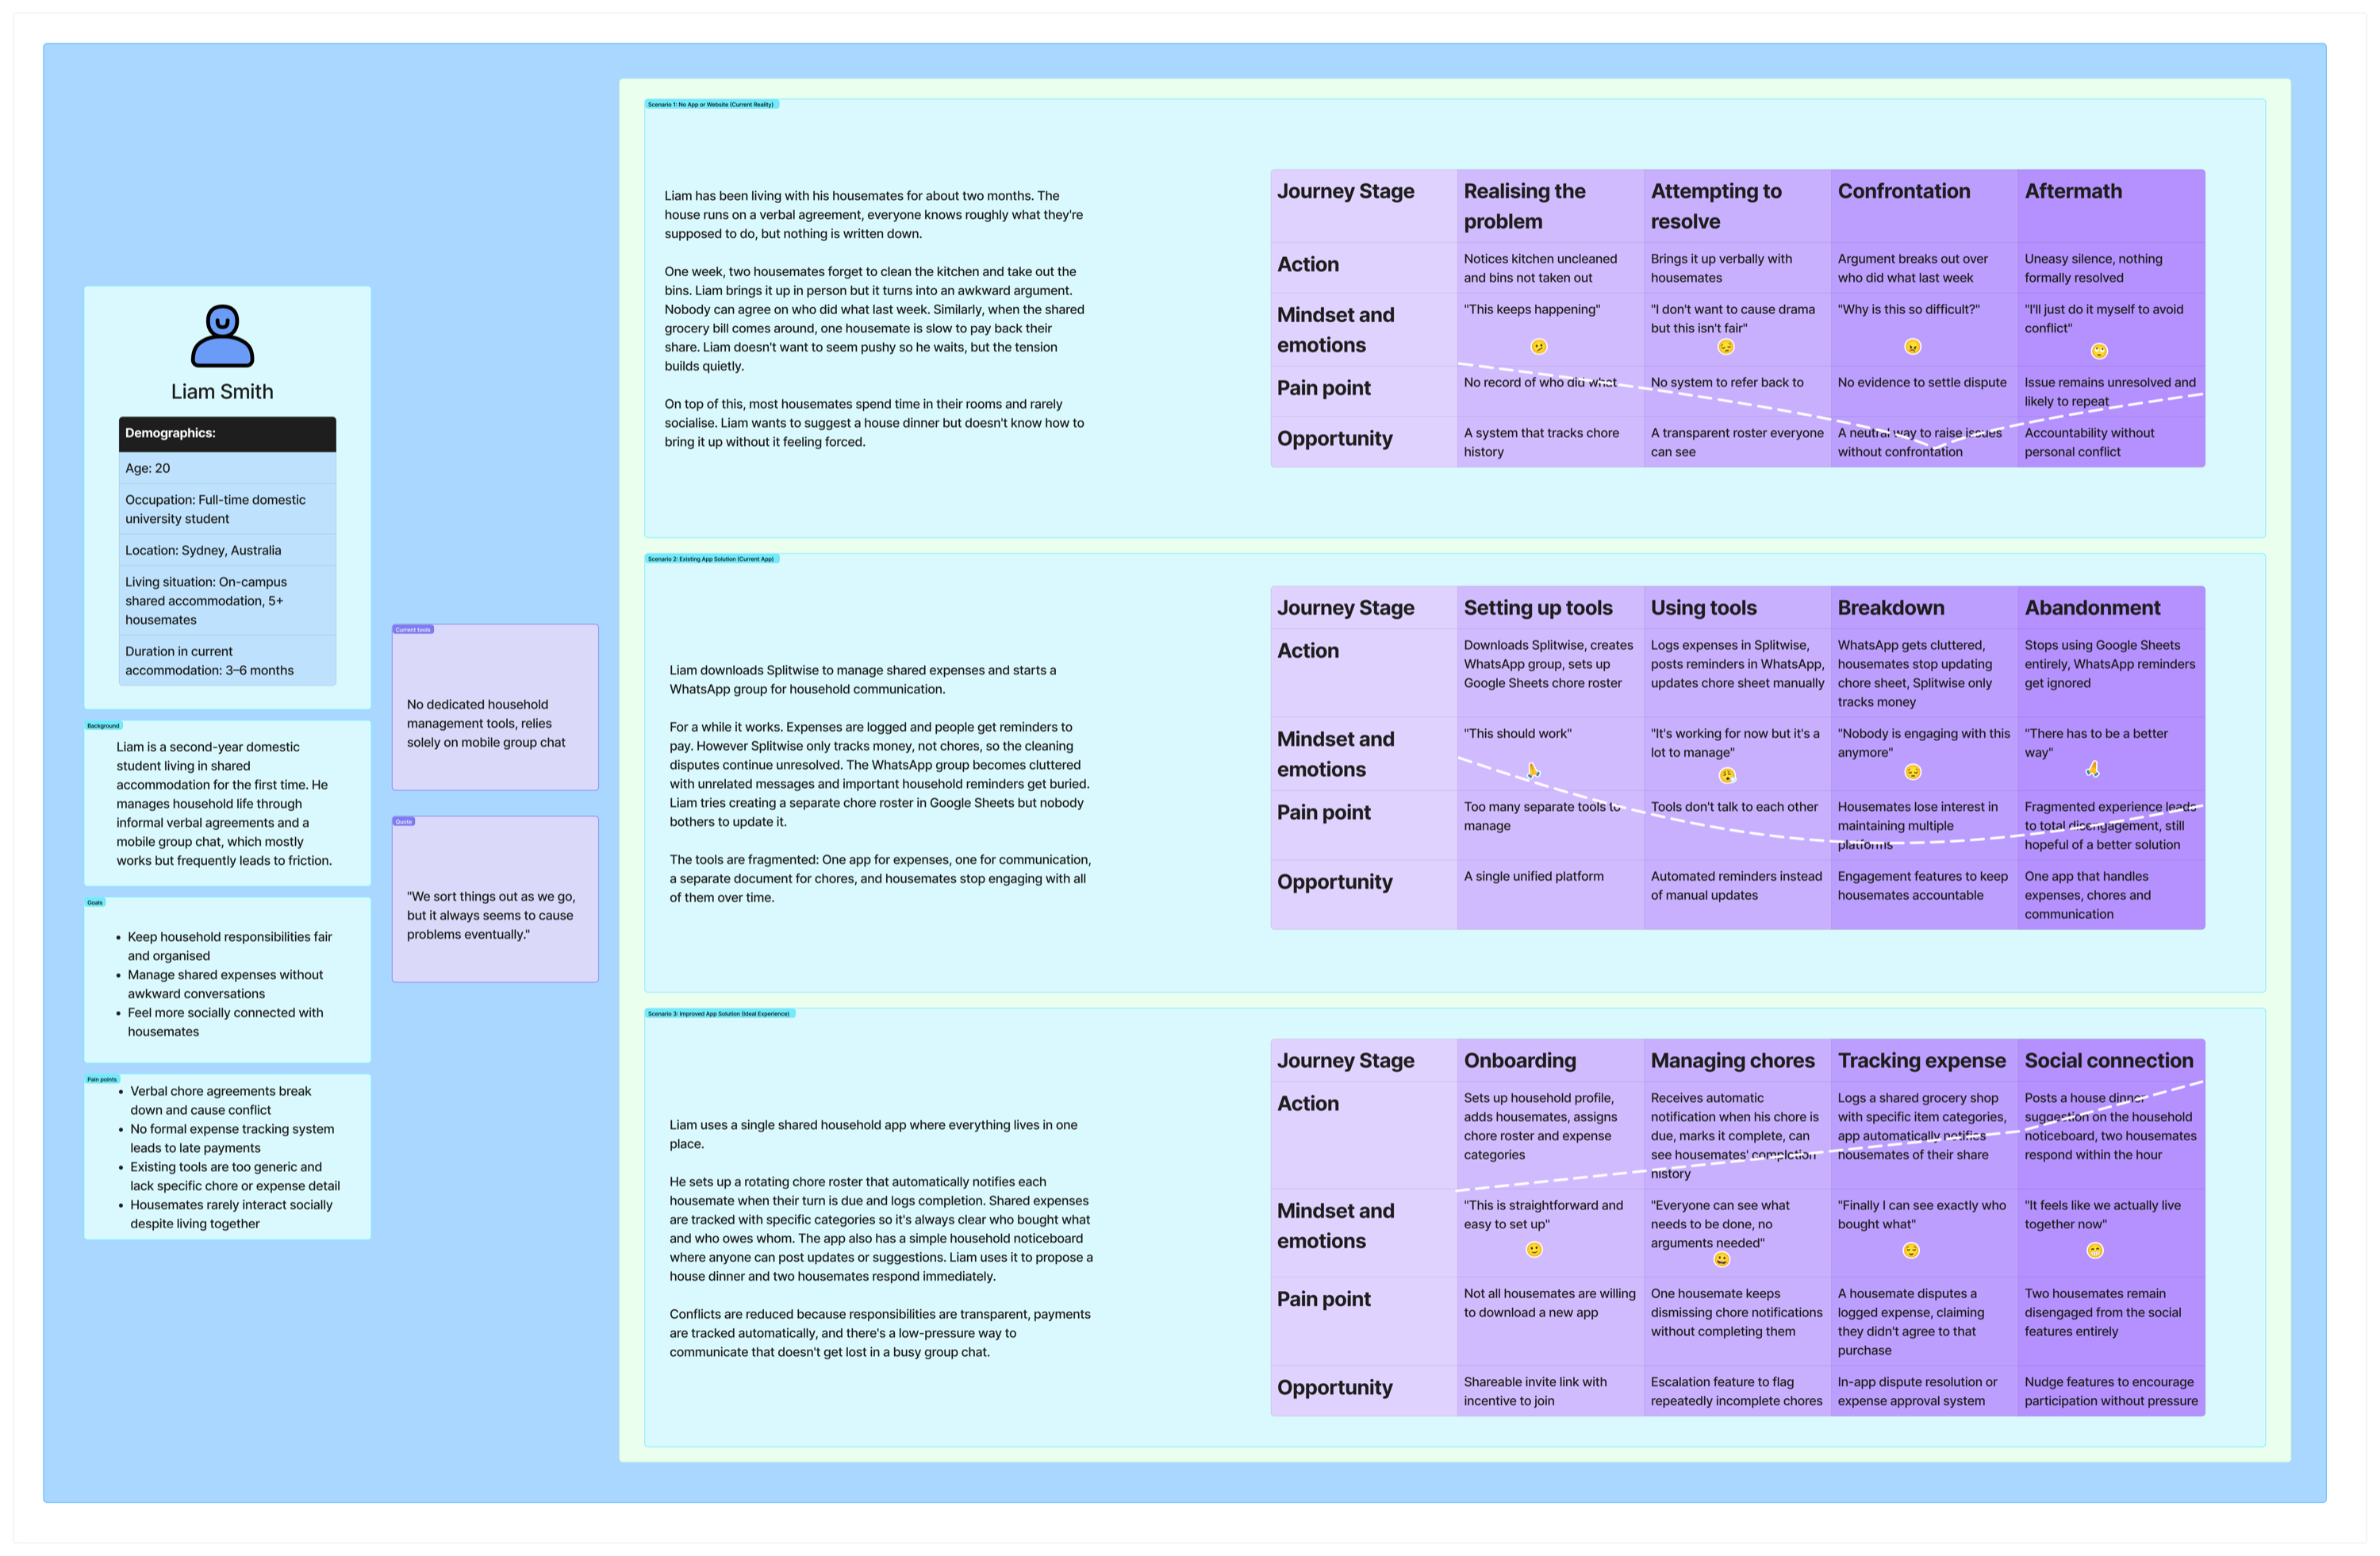
\includegraphics[width=\textwidth,height=0.48\textheight,keepaspectratio]{domestic_student_persona_liam_smith.png}
    \caption{Liam Smith domestic shared living student persona, scenarios and journey maps.}
    \label{figdomesticpersona}
\end{figure}

The property manager persona represents a secondary stakeholder who shapes the trust environment around student accommodation. This persona is not the primary design target, but it shows why verified listing details, structured applicant information and guided communication matter. The journey map shows that property managers face repeated enquiries, incomplete applications and pressure to assess tenant suitability efficiently.

\begin{figure}[H]
    \centering
    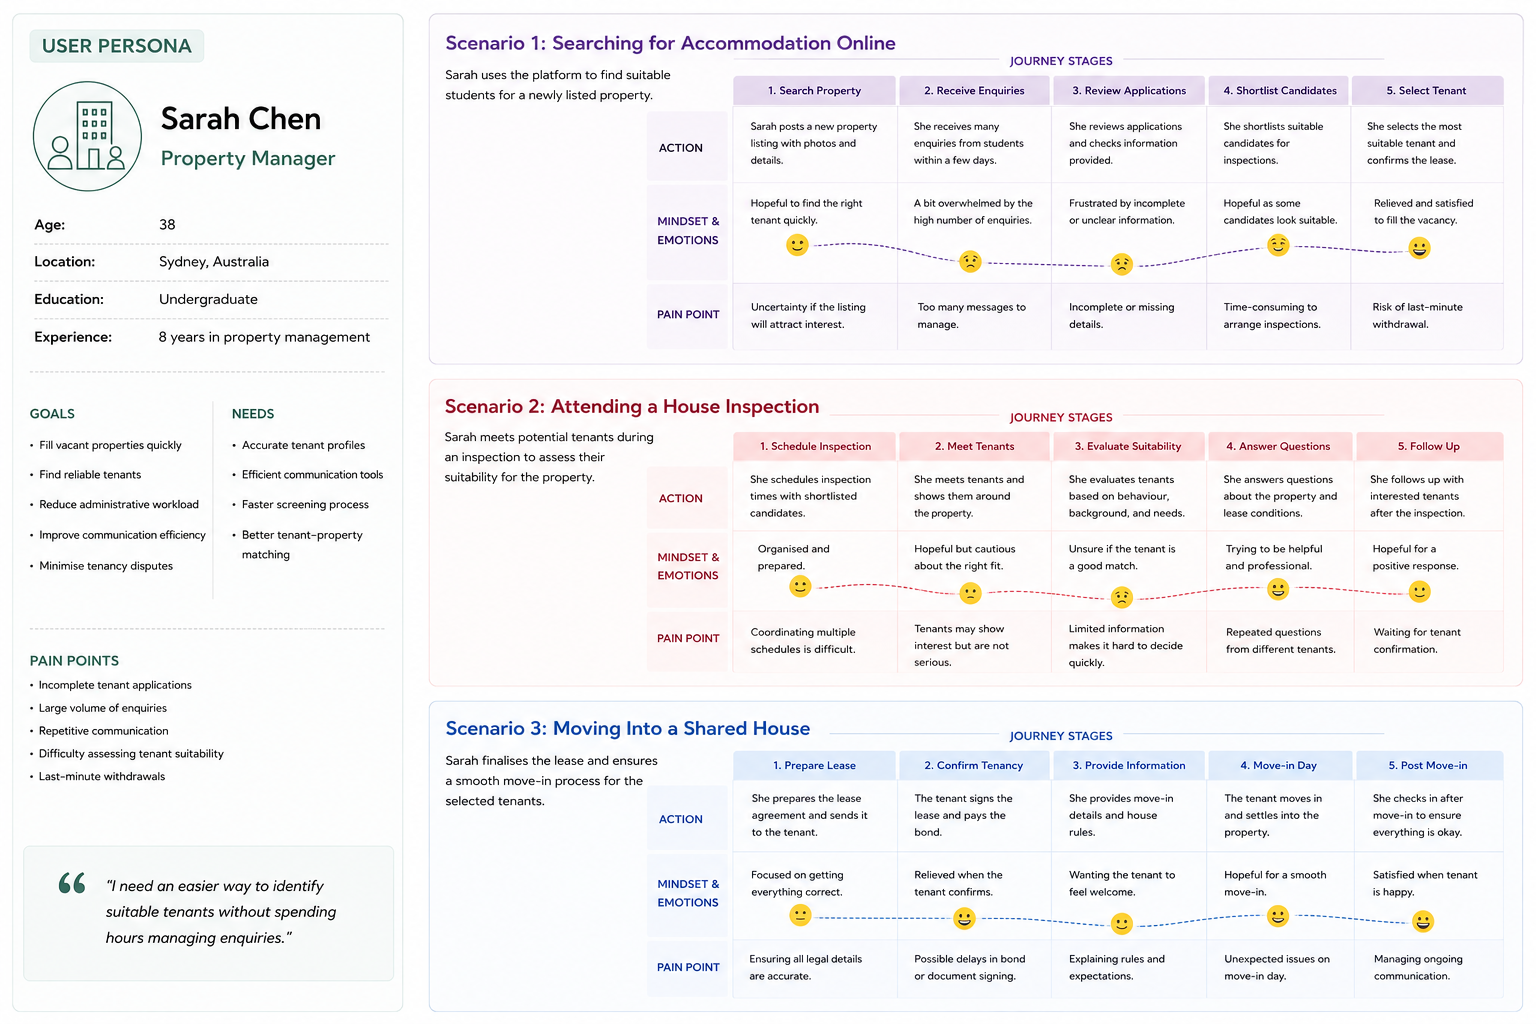
\includegraphics[width=\textwidth,height=0.48\textheight,keepaspectratio]{property_manager_persona.png}
    \caption{Property manager persona, scenario and journey map.}
    \label{figpropertymanagerpersonamain}
\end{figure}

These four personas show that the project should not only help students find accommodation. It should help them make a safer and more informed commitment. The design should therefore support verified listing information, structured housemate profiles, compatibility comparison, guided communication and early clarification of shared responsibilities.

\section{Common Goals and Pain Points}

The synthesis table links user goals with the problems found in the research and the design direction that follows from them.

\begin{table}[H]
    \centering
    \small
    \caption{Common goals and pain points synthesised across user research.}
    \begin{tabularx}{\textwidth}{@{}L{3.1cm} Y L{3.0cm} Y@{}}
        \toprule
        Common goal & Pain point & Evidence source & Design implication\\
        \midrule
        Find safe accommodation & Users struggle to judge whether a listing is genuine. & International survey and interview & The product should help users check listing identity and evidence.\\
        Choose suitable housemates & Lifestyle habits are hard to see before commitment. & Survey, interview and Emily Chen persona & Profiles should ask about routines and expectations in plain terms.\\
        Communicate clearly & Replies may arrive late or miss information users need. & Interview and accommodation search journey map & Messaging should guide the questions users need to ask.\\
        Avoid future conflict & Household work, bills and rules are often not discussed early enough. & Domestic survey & The experience should surface shared expectations before move in.\\
        Decide with confidence & Users feel pressure when evidence is incomplete. & Journey maps & The product should help users compare options and review expectations before deciding.\\
        \bottomrule
    \end{tabularx}
    \label{tabgoals}
\end{table}

\section{Problem Definition}

\subsection{Convergence From Research}

The team first explored trust in rentals, how housemates communicate, how household responsibilities are shared and how conflict develops. Survey and interview findings showed that many of these concerns connect to an earlier decision point. Students and shared-house residents often commit to accommodation or housemates before they have enough reliable information about listing legitimacy, lifestyle fit and responsibility expectations. The team therefore focused on the stage where users evaluate accommodation and housemates before commitment.

\begin{figure}[H]
    \centering
    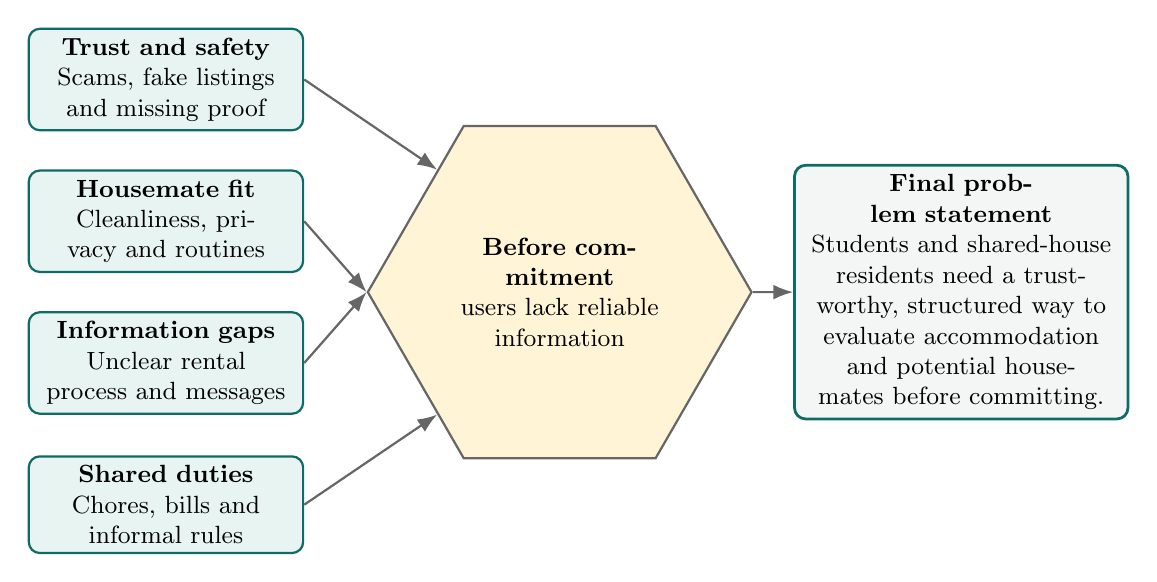
\begin{tikzpicture}[
        font=\small,
        theme/.style={
            draw=accent,
            fill=softaccent,
            rounded corners=4pt,
            line width=0.8pt,
            text width=3.25cm,
            align=center,
            minimum height=1.15cm
        },
        synthesis/.style={
            draw=midgray,
            fill=softgold,
            regular polygon,
            regular polygon sides=6,
            line width=0.8pt,
            text width=2.75cm,
            align=center,
            minimum size=2.45cm
        },
        outcome/.style={
            draw=accent,
            fill=softgray,
            rounded corners=4pt,
            line width=1pt,
            text width=4.0cm,
            align=center,
            minimum height=2.1cm
        },
        arrow/.style={-{Latex[length=2.5mm]}, line width=0.8pt, draw=midgray}
    ]
        \node[theme] (trust) at (0,2.7) {\textbf{Trust and safety}\\Scams, fake listings and missing proof};
        \node[theme] (fit) at (0,0.9) {\textbf{Housemate fit}\\Cleanliness, privacy and routines};
        \node[theme] (communication) at (0,-0.9) {\textbf{Information gaps}\\Unclear rental process and messages};
        \node[theme] (responsibility) at (0,-2.7) {\textbf{Shared duties}\\Chores, bills and informal rules};

        \node[synthesis] (converge) at (5.0,0) {\textbf{Before commitment}\\users lack reliable information};
        \node[outcome] (problem) at (10.1,0) {\textbf{Final problem statement}\\Students and shared-house residents need a trustworthy, structured way to evaluate accommodation and potential housemates before committing.};

        \draw[arrow] (trust.east) -- (converge.north west);
        \draw[arrow] (fit.east) -- (converge.west);
        \draw[arrow] (communication.east) -- (converge.west);
        \draw[arrow] (responsibility.east) -- (converge.south west);
        \draw[arrow] (converge.east) -- (problem.west);
    \end{tikzpicture}
    \caption{Convergence diagram linking research themes to the final problem definition.}
    \label{figconvergence}
\end{figure}

\subsection{Final Problem Statement}

International students and new shared house residents need a trustworthy and structured way to evaluate accommodation and potential housemates before committing. Existing search and communication processes make it difficult to check whether a listing is legitimate, compare lifestyle fit and discuss who cleans, how bills are paid, how privacy is handled and what the household expects.

\subsection{Justification}

This problem matters because it appears before users make a risky housing decision and then shapes their living experience. The research showed that trust concerns, unclear compatibility and informal expectations can lead to anxiety, poor decisions and conflict after move in. A focused problem definition gives the next design phase a clear direction. The solution should let users check whether a listing can be trusted, understand how a potential housemate lives, communicate through a guided flow and agree on expectations before moving in.

\section{Conclusion}

Through stakeholder analysis, surveys, interviews, and personas, the team identified that students and shared-house residents need better support before committing to a room or housemate. The findings highlight the importance of trust, communication, and compatibility during the accommodation search process. These insights will guide the next stage of the project, where potential design solutions will be developed and evaluated.

\newpage
\section{References}

\begingroup
\small
\sloppy
\begin{itemize}
    \item Liam and Cara. (2026). Primary research interview for the accommodation app project. YouTube video: \url{https://www.youtube.com/watch?v=hysLiuMwqtg}.
    \item Clark, V., Tuffin, K., Frewin, K. \& Bowker, N. (2018). Housemate desirability and understanding the social dynamics of shared living. \textit{Qualitative Psychology}, 5(1), 26--40.
    \item UNSW Human Rights Clinic. (2019). \textit{No Place Like Home: Addressing Exploitation of International Students in Sydney's Housing Market}. UNSW Sydney. \url{https://www.law.unsw.edu.au/sites/default/files/imce/files/UNSW0006-No-Place-Like-Home_Executive-Summary.pdf}.
    \item Goodall, Z. \& Stone, W. (2024). Sharing risk in shared housing: Rental regulations and housing justice in Australia. \textit{International Journal of Housing Policy}. \url{https://doi.org/10.1080/19491247.2024.2367836}.
    \item Goodall, Z., Stone, W., Cook, K. \& Batterham, D. (2025). Understanding housing justice in shared housing. \textit{Housing, Theory and Society}, 1--18. \url{https://doi.org/10.1080/14036096.2025.2562110}.
    \item Domestic Student Shared Housing Experience Survey results. (2026). Week 2 primary survey data. SurveyMars. \url{https://surveymars.com/app/survey/analyze/results/default/druhESmaB}.
    \item Interaction Design Foundation. (2025). \textit{Personas: A Simple Introduction}. \url{https://www.interaction-design.org/literature/article/personas-why-and-how-you-should-use-them}.
\end{itemize}
\endgroup

\appendix
\section{Interview Evidence}

The interview asked why accommodation search feels frustrating and why very cheap social media listings can appear risky. It also explored what the participant wanted to know about a place and the people living there, including cleanliness, privacy, photos, reviews and roommate ratings. The evidence source is the team interview video on YouTube: \url{https://www.youtube.com/watch?v=hysLiuMwqtg}.

\begin{table}[H]
    \centering
    \small
    \caption{Interview evidence summary.}
    \begin{tabularx}{\textwidth}{@{}L{3.8cm} Y Y@{}}
        \toprule
        Topic & Interview insight & Use in report\\
        \midrule
        Trust & Very cheap social media listings can feel suspicious when the information is incomplete. & Supports the trust and safety finding.\\
        Compatibility & Cleanliness, privacy and schedule fit were treated as practical shared living needs. & Supports the Emily Chen general resident persona.\\
        Listing information & The participant expected location details, realistic photos, reviews and information about nearby facilities before deciding. & Supports the communication and information gap finding.\\
        \bottomrule
    \end{tabularx}
\end{table}

\section{International Student Survey Evidence}

The international student survey included 16 valid responses. The evidence showed how students perceived scams, how much compatibility mattered and what problems they faced before arrival. It also covered experiences with misleading listings and expectations for platform features. The full survey report is stored in the repository as \textit{International Student Accommodation Search Experience Survey in Australia - Default Report.pdf}.

\begin{table}[H]
    \centering
    \small
    \caption{International survey evidence summary.}
    \begin{tabularx}{\textwidth}{@{}L{4.0cm} Y Y@{}}
        \toprule
        Evidence & Result & Report implication\\
        \midrule
        Rental scam concern & 16 out of 16 respondents reported concern, and 50\% were very concerned. & Trust checking is a core need.\\
        Misleading listing experience & 43.75\% had experienced misleading or false information in a housing advertisement. & Verification should address real user experience, not only perceived risk.\\
        Compatibility importance & The average score was 4.44 out of 5, and 87.5\% rated compatibility as very or extremely important. & Matching should include lifestyle expectations.\\
        Search challenge before arrival & Language barriers were the most selected difficulty at 43.75\%. & Guided communication should reduce uncertainty.\\
        Platform expectation & 81.25\% would probably or definitely use a preference-based roommate matching platform. & The concept has early evidence of user acceptance.\\
        \bottomrule
    \end{tabularx}
\end{table}

\section{Domestic Student Shared Living Survey Evidence}

The domestic student shared living survey included 3 valid responses. The evidence covered how students manage household work, how conflict appears around responsibilities, how bills are split, how late payments occur and how housemate connection develops. Because the sample is small, the results are used as supporting evidence alongside the Liam Smith persona and secondary shared housing sources. The full survey report is stored in the repository as \textit{Domestic Student Shared Housing Experience Survey - Default Report.pdf}.

\begin{table}[H]
    \centering
    \small
    \caption{Domestic survey evidence summary.}
    \begin{tabularx}{\textwidth}{@{}L{4.0cm} Y Y@{}}
        \toprule
        Evidence & Result & Report implication\\
        \midrule
        Household work management & 100\% used verbal informal agreements. & Informal systems are fragile.\\
        Household responsibility conflict & 100\% had experienced conflict. & Expectations should be clarified before move in.\\
        Bill splitting & 66.67\% had no formal bill splitting arrangement. & Compatibility should include expectations around shared responsibilities.\\
        Expense payment issues & 100\% had experienced issues with housemates not paying their share on time. & Shared expense tracking and reminders are important design opportunities.\\
        Communication tools & 100\% used mobile group chat, while 0\% used a chore management app. & Current tools support conversation but not accountability.\\
        \bottomrule
    \end{tabularx}
\end{table}

\section{Team Synthesis Artefact}

\begin{figure}[H]
    \centering
    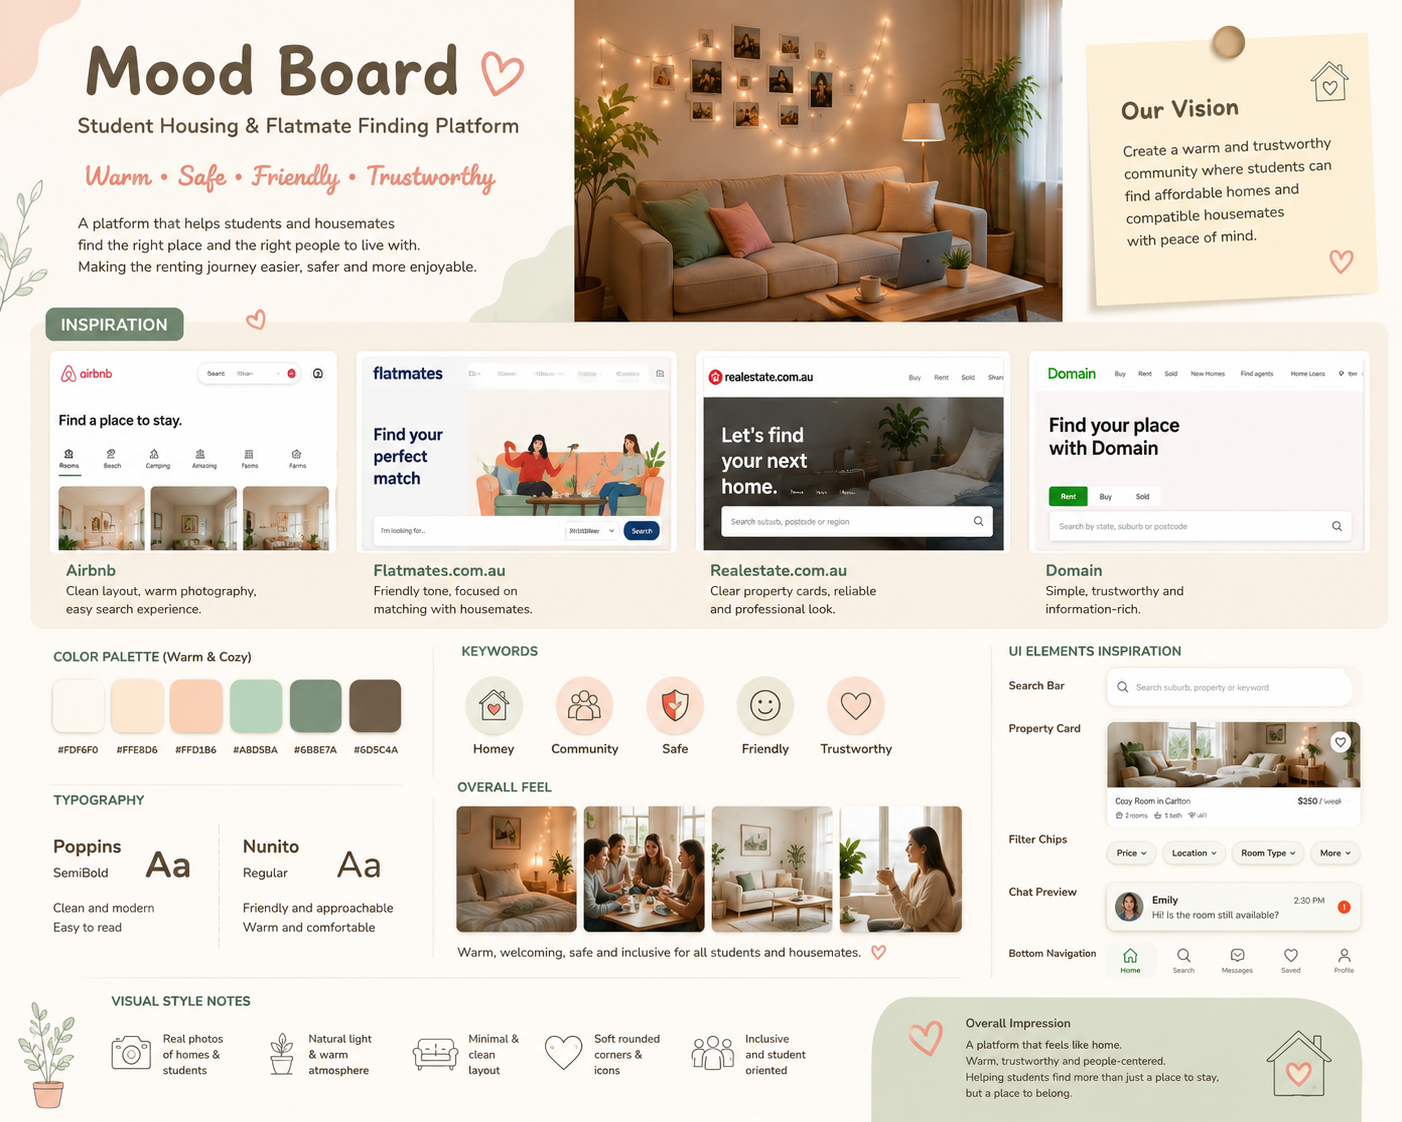
\includegraphics[width=\textwidth,height=0.7\textheight,keepaspectratio]{../desn2000-moodboard.png}
    \caption{Week 4 team mood board synthesis artefact.}
    \label{figmoodboard}
\end{figure}

\section{Meeting Minutes}

The meeting minutes are stored in the public GitHub repository so the report can reference the team's weekly planning and progress evidence without relying on private workspace links.

\begin{table}[H]
    \centering
    \small
    \caption{Meeting minutes evidence links.}
    \begin{tabularx}{\textwidth}{@{}L{2.4cm} Y Y@{}}
        \toprule
        Week & GitHub evidence link & Evidence purpose\\
        \midrule
        Week 1 & \href{https://github.com/NuodiLiu/DESN2000/blob/main/meeting_minutes/week1.txt}{meeting\_minutes/week1.txt} & Initial stakeholder identification, task allocation and research planning.\\
        Week 2 & \href{https://github.com/NuodiLiu/DESN2000/blob/main/meeting_minutes/week2.txt}{meeting\_minutes/week2.txt} & Interview, persona, user story and progress planning.\\
        Week 3 & \href{https://github.com/NuodiLiu/DESN2000/blob/main/meeting_minutes/week3.txt}{meeting\_minutes/week3.txt} & Persona, journey map, Jira and report assembly progress.\\
        Week 4 & \href{https://github.com/NuodiLiu/DESN2000/blob/main/meeting_minutes/week4.txt}{meeting\_minutes/week4.txt} & Week 4 meeting record file in the project repository.\\
        \bottomrule
    \end{tabularx}
\end{table}

\end{document}
